\documentclass[12pt,a4paper]{article}
\title{%
  Øving 9 \\
  \large IELET1001 - Elektroteknikk \\
  }
\author{Gunnar Myhre, BIELEKTRO}

\usepackage[utf8]{inputenc}
\usepackage[norsk]{babel}
\usepackage[siunitx]{circuitikz}
\usepackage{amsmath}

\usepackage{graphicx}
\graphicspath{ {./images} }

\setlength\parindent{0pt}

\begin{document}
  \maketitle

  \section*{Oppgåve 1}
    \subsection*{a)}
    Omgjer $i(t)$ til kanonisk form
    \begin{equation}
      i(t) = 3sin(\omega t) = 3cos(\omega t - \ang{90})
    \end{equation}
    setter inn i formel for gjennomsnittleg effekt
    \begin{equation}
      P = \frac{1}{2}V_mI_m cos(\theta _v - \theta _i)
    \end{equation}
    \begin{equation}
      P =  \frac{22\cdot3}{2}cos(0-\ang{90}) = 0W
    \end{equation}

    \subsection*{b)}
    Omgjer $i(t)$ til kanonisk form
    \begin{equation}
      i(t) = 5sin(\omega t + \ang{45}) = 5cos(\omega t - \ang{45})
    \end{equation}
    setter inn i formel for gjennomsnittleg effekt
    \begin{equation}
      P = \frac{1}{2}V_mI_m cos(\theta _v - \theta _i)
    \end{equation}
    \begin{equation}
      P = \frac{170\cdot5}{2}cos(\ang{30}-(\ang{-45})) = 110 W
    \end{equation}


  \section*{Oppgåve 2}
    Finner $Z_{ekv}$
    \begin{equation}
      Z_{ekv} = \left( (2-2j) || 2j \right) + 4 = \frac{2j(2-2j)}{2j+(2-2j)} + 4
    \end{equation}
    \begin{equation}
      Z_{ekv} = j(2-2j) + 4 = 6+2j
    \end{equation}
    skriver $Z$ på polar form
    \begin{equation}
      Z = 6+2j = \sqrt{6^2 + 2^2}\angle arctan \left( \frac{2}{6} \right) =
      6,34\angle \ang{18,4}
    \end{equation}
    finner $I$
    \begin{equation}
      I=\frac{V}{Z} = \frac{12\angle \ang{60}}{6,34 \angle \ang{18,4}} =
      1,89\angle \ang{41,6}
    \end{equation}
    setter inn i formel for momentaneffekt
    \begin{equation}
      p(t) = \frac{V_m I_m}{2} \left[ cos(\theta _v - \theta _i) +
      cos(2\omega t + \theta _v + \theta _i ) \right] 
    \end{equation}
    \begin{equation}
      p(t) = 11,34\cdot0,95 + 11,34\cdot cos(2\omega t + \ang{60} + \ang{41,6})
    \end{equation}
    \begin{equation}
      p(t) = 10,82 + cos(2\omega t + \ang{101,6}) [W]
    \end{equation}

  \newpage

  \section*{Oppgåve 3}
    Gjer om alle mengdene til det komplekse domenet
    \begin{itemize}
      \item $60mH \longrightarrow Z_L = j\omega L = j120$
      \item $12,5\si{\micro\farad} \longrightarrow Z_C = \frac{1}{j\omega C} = -j40$
      \item $i(t) = 0,5cos(2000t) \longrightarrow 0,5\angle \ang{0}$
    \end{itemize}
    \begin{center}
      \begin{circuitikz}[american] \draw
        (0,0) to[I, l=$I$, v=$V$] (0,4) -- (2,4)
              to[R, l=$40$] (4,4)
              to[L, l=$j120$, i=$I_b$] (4,0) -- (0,0)
        (2,0) to[C, l=$-j40$, i<=$I_a$] (2,2)
              to[R, l=$130$] (2,4)
        ;
      \end{circuitikz}
    \end{center}
    finner $I_a$ og vha. straumdeling
    \begin{equation}
      I_a = \frac{40+j120}{170+j80}I = 0,232+j0,244 = 0,337\angle \ang{46,4}
    \end{equation}
    \begin{equation}
      I_b = I-I_a = 0,268 -j0,244 = 0,354\angle \ang{-42,3}
    \end{equation}
    finner spenningene over komponentene
    \begin{itemize}
      \item $V_{130} = Z_{130}I_{a} = 130\cdot0,337\angle \ang{46,4} = 43,81\angle \ang{46,4}$
      \item $V_{40} = Z_{40}I_{b} = 40\cdot0,354\angle \ang{-42,3} = 14,16\angle \ang{-42,3}$
      \item $V = Z_{ekv}I = \frac{(40+120j)(130-40j)}{170+80j}I = 45,79\angle\ang{29,26}$
    \end{itemize}
    finner den aktive gjennomsnittseffekten. Dei reaktive kretselementene forbruker ingen
    aktiv effekt så vi ser bort ifrå dei.
    \begin{itemize}
      \item $P_{130} = \frac{V_{130}I_a}{2}cos(\theta_v - \theta_i)
        = \frac{43,81\cdot0,337}{2} \cdot cos(\ang{0}) = 7,38[W]$
      \item $P_{40} = \frac{V_{40}I_b}{2}cos(\theta_v - \theta_i)
        = \frac{14,16\cdot0,354}{2} \cdot cos(\ang{0}) = 2,51[W]$
      \item $P = \frac{V(-I)}{2}cos(\theta_v - \theta_i) =
        \frac{45,79\cdot(-0,5)}{2}cos(29,26) = -9,987[W]$
    \end{itemize}

  \section*{Oppgåve 4}
    Finner theveninekvivalenten
    \begin{equation}
      Z_{th} = 2+j2[\si{\ohm}]
    \end{equation}
    kjeldetransformerer for å finne $V_{th}$
    \begin{equation}
      V_{th} = 2\cdot 16\angle \ang{0}
    \end{equation}
    vi veit at $Z_L$ må vere den komplekskonjugerte av $Z_{th}$ for å oppnå
    maksimal effektoverføring. Derfor setter vi $Z_L = (2-j2)[\si{\ohm}]$. Effekten i forbrukt
    i denne lasta er dermed 
    \begin{equation}
      P_L = \frac{V_L I_L}{2\sqrt{2}} cos(\theta_v - \theta_i) = 63,64 [W]
    \end{equation}
    eg deler på $\sqrt{2}$ for å få RMS-verdi

  \section*{Oppgåve 5}
    RMS-verdien er gitt som
    \begin{equation}
      V_{rms} = \sqrt{\frac{1}{T} \int_{t_0}^{t_0 + T} V^2 dt}
    \end{equation}
    i dette tilfellet ser vi at arealet under $v(t)$ i løpet av ein periode $T=6$ er $10$,
    då får vi
    \begin{equation}
      V_{rms} = \sqrt{\frac{10^2}{6}} = 4,08 [V_{rms}]
    \end{equation}


  \section*{Oppgåve 6}
    Finner RMS-verdien for spenninga
    \begin{equation}
      V_{rms} = \sqrt{\frac{1}{T} \int_{t_0}^{t_0 + T} V^2 dt}
      \rightarrow
      V_{rms} = \sqrt{\frac{1}{2\pi} \int_{0}^{\pi} 10^2sin^2(t)dt} = \sqrt{25} = 5 [V_{rms}]
    \end{equation}
    finner effekten forbrukt av motstanden
    \begin{equation}
      P = \frac{V^2}{R} = \frac{25}{10} = 2,5 [W_{rms}]
    \end{equation}


  \section*{Oppgåve 7}
    \subsection*{a)}
    Vi kan finne effektfaktoren vha. formel for kompleks effekt
    \begin{equation}
      S = V_{rms}I_{rms}\cdot pf \rightarrow pf = \frac{S}{V_{rms}I_{rms}}
      \rightarrow pf = \frac{90\cdot 10^3}{260\cdot480} = 0,7212
    \end{equation}
    Vi veit at effekten er bakpå (\textit{lagging}) sidan lasta er induktiv

    \subsection*{b)}
    Setter inn i formel for kompleks effekt
    \begin{equation}
      S = V_{rms}I_{rms}\cdot pf \rightarrow V_{rms} = \frac{S}{pf\cdot I_{rms}}
      \rightarrow V_{rms} = 568,2[V_{rms}]
    \end{equation}

  \section*{Oppgåve 8}
    \subsection*{a)}
    \begin{center}
      \begin{circuitikz}[american] \draw
        (0,0) to[generic, l=$Z_L$, i=$i(t)$, v=$v(t)$, *-*] (4,0)
        ;
      \end{circuitikz}
    \end{center}
    Effektfaktoren er gitt som
    \begin{equation}
      pf = cos(\theta_v - \theta_i) = cos(\ang{-20}-\ang{10}) = 0,866
    \end{equation}
    sidan $\theta_z$ er mindre enn 0 er lasta kapasitiv, og effekten er derfor
    frampå (\textit{leading}).

    \subsection*{b)}
    Finner impedansen til lasta vha. Ohms lov
    \begin{equation}
      Z_L = \frac{V}{I} = \frac{120\angle\ang{-20}}{4\angle\ang{10}} = 30\angle\ang{-30}
      = 25,98 - 15j
    \end{equation}
    finner kapasitansen vha. definisjonen av fasevektor for kondensator
    \begin{equation}
      Z = \frac{1}{j\omega C} \rightarrow C_L = \frac{-j}{\omega Z_L} \rightarrow
      C = \frac{1}{15\cdot100\pi} = 212,2\si{\micro\farad}
    \end{equation}
    resistansen til lasta er den reale delen, $R_L = 25,98\si{\ohm}$


  \section*{Oppgåve 9}
    Finner $Z_{ekv}$
    \begin{equation}
      Z_{ekv} = ((6||-j2)+3+j4)||5 = \left(\frac{18}{5}+j\frac{11}{5} \right) || 5
      = 2,272 + 0,698j = 2,377\angle\ang {17,08}
    \end{equation}
    finner RMS-verdien for straumkjelda
    \begin{equation}
      I_{rms} = \frac{2}{\sqrt{2}}
    \end{equation}
    finner den komplekse effekten
    \begin{equation}
      S = I_{rms}^2Z = \left(\frac{2}{\sqrt{2}}\right)^2 \cdot 2,377\angle\ang{17,08}
      = 4,754 \angle\ang{17,08}
    \end{equation}
    på kartesisk form er den komplekse effekten
    \begin{equation}
      S = 4,544 + j1,396 [VA]
    \end{equation}


  \section*{Oppgåve 10}
    Informasjonen som er gitt i oppgåveteksten:
    \begin{itemize}
      \item tilsynelatande effekt $ = 12[kVA]$
      \item $pf = 0,856$
      \item lagging $\rightarrow$ induktiv
      \item $V_{rms} = 120[V_{rms}]$
    \end{itemize}

    \subsection*{a)}
    Finner $I_{rms}$
    \begin{equation}
      I_{rms}V_{rms} = 12000[VA] \rightarrow I_{rms} = 100[A_{rms}]
    \end{equation}
    finner den aktive effekten
    \begin{equation}
      P = 12\cdot 10^3 \cdot 0,856 = 10272[W]
    \end{equation}
    for å finne den reaktive effekten må vi finne $\theta_z$
    \begin{equation}
      pf = cos(\theta_z) \rightarrow \theta_z = arccos(pf) = \ang{31,13}
    \end{equation}
    den reaktive effekten er
    \begin{equation}
      Q = VAsin(\theta_z) = 12000\cdot sin(\ang{31,13}) = 6204[VAR]
    \end{equation}

    \subsection*{b)}
    \begin{equation}
      I_M = I_{rms}\sqrt{2} = 141,4[A]
    \end{equation}

    \subsection*{c)}
    Nå som vi kjenner den komplekse effekten kan vi enkelt finne lastimpedansen
    \begin{equation}
      S = I_{rms}^2 Z \rightarrow Z_L = \frac{10272+6402j}{100^2} = 1,0272 + 0,6204j[\si{\ohm}]
    \end{equation}

  \section*{Oppgåve 11}
    Sidan effektfaktoren er bakpå (lagging) veit vi at lasta $Z_L$ er induktiv, og vi
    ønsker derfor å legge til ein kondensator $Z_K$ for å kompansere for litt av
    reaktansen og heve effektfaktoren frå $0,8$ til $0,9$.
    Slik ser kretsen ut etter at kompensasjonsimpedansen er kopla til.
    \begin{center}
      \begin{circuitikz}[american] \draw
        (0,0) to[V, l=$V$, i>=$I$, invert] (0,2) -- (3,2)
              to[generic, l=$Z_L$, *-*] (3,0) --(0,0)
        (2,0) to[generic, l=$Z_K$] (2,2)
        ;
      \end{circuitikz}
    \end{center}
    Etter mykje prøving og feiling viser det seg at dette ganske enkelt lar seg løyse
    som eit trigonometrisk problem dersom vi teikner opp ein trikant som viser forholdet
    mellom kompleks effekt \textbf{S}, aktiv effekt \textbf{P=40\si{\kilo\watt}} og
    reaktiv effekt \textbf{Q}, sidan dei er akser i det komplekse planet.
    \begin{equation}
      S = P + jQ
    \end{equation}
    Vinkelen til denne trikanten er gitt ved effektfaktoren 
    \begin{equation}
      pf = cos(\theta) \longrightarrow \theta = arccos(0,8) = \ang{36,86}
    \end{equation}
    Den effektfaktoren vi ønsker å oppnå bestemmer også ein vinkel $\theta_{ny}$
    \begin{equation}
      pf_{ny} = cos(\theta_{ny}) \longrightarrow \theta_{ny} = arccos(0,9) = \ang{25,84}
    \end{equation}
    så kun ved hjelp av dei oppgitte mengdene $P$ og $pf = 0,8$ kan vi teikne opp trikanten
    \begin{center}
      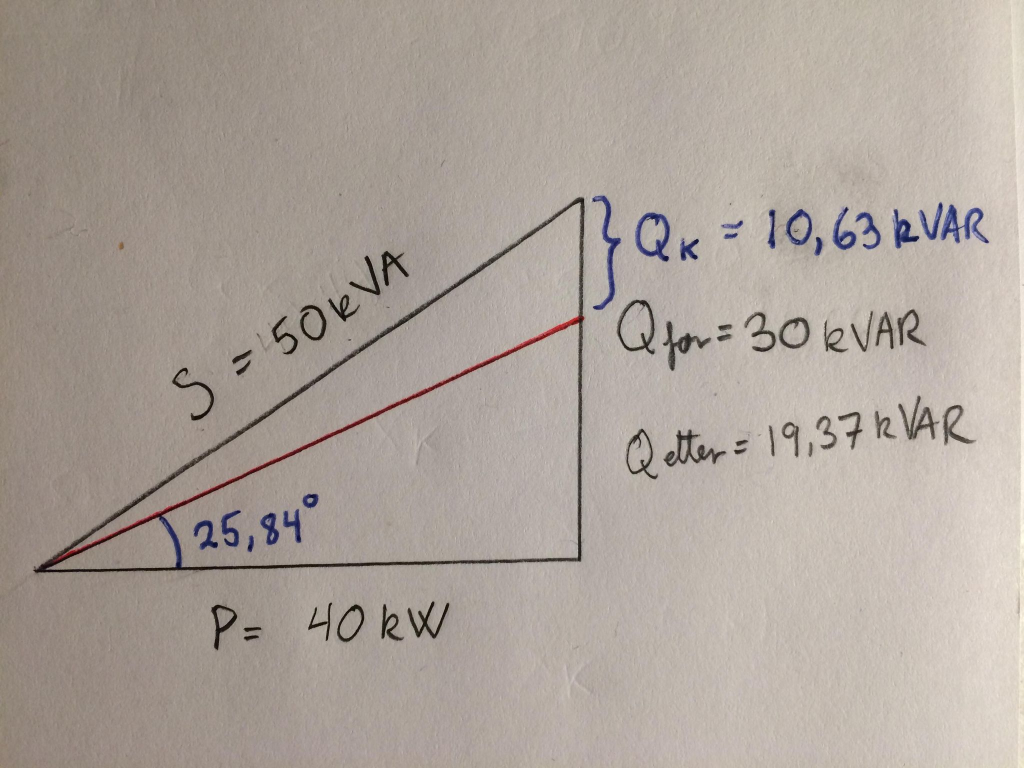
\includegraphics[scale=0.3]{09_pf.png}
    \end{center}
    Vi har nok informasjon til å rekne ut alle mengdene av $Q$, som vi er ute etter.
    \begin{itemize}
      \item $tan(\theta) = \frac{mot}{hos} \rightarrow Q_{før} = 40kW\cdot tan(\ang{36,86})
        = 30kVAR$
      \item $Q_{etter} = 40kW\cdot tan(\ang{25,84}) = 19,37kVAR$
      \item $Q_K = Q_{før} - Q_{etter} = 10,63kVAR$
    \end{itemize}
    Sidan vi kjenner til at spenninga over kondensatoren $Z_K$ er $V=220$ kan vi finne
    reaktansverdien $X_K$ slik
    \begin{equation}
      Q_K = \frac{V^2}{X_K} \rightarrow X_K = \frac{220^2}{10,63\cdot10^3} = 4,553\si{\ohm}
    \end{equation}
    frekvensen $60Hz$ kan vi oversette til vinkelfrekvens på denne måten
    \begin{equation}
      f = \frac{\omega}{2\pi} \rightarrow \omega = 2\pi60
    \end{equation}
    nå kan vi finne kapasitansen $C_K$
    \begin{equation}
      X_K = \frac{1}{\omega C} \rightarrow C_K = \frac{1}{120\pi4,553} = 5,825 \cdot 10^{-4}
    \end{equation}
    Kapasitansen må vere $583 \si{\micro\farad}$ for å få den ønska effektfaktoren.
\end{document}
